
\providecommand{\main}{..} 
\documentclass[\main/notes.tex]{subfiles} 

\begin{document} 
\begin{center} 
\textbf{{\Large Simulation Parameters}} 
\end{center} 

Recently,~\citet{Spitoni2021} parameterized the two-infall model for three 
bins in radius in the Galactic disk. 
The infall history is given by: 
\begin{equation} 
\dot{M}_\text{in} = N_1 e^{-t / \tau_1} + H(t - \tmax) N_2 
e^{-(t - \tmax) / \tau_2} 
\end{equation} 
where~$N_1$ and~$N_2$ are coefficients describing the normalization of the two 
exponentials,~$\tau_1$ and~$\tau_2$ are the associated e-folding 
timescales,~\tmax~is the time of onset of the second exponential, and~$H$ is the 
Heaviside step function. 
They used MCMC methods to obtain best-fit values for these parameters; however, 
they instead report the present-day surface denisities of high- and low-$\alpha$ 
stars~$\sigma_1$ and~$\sigma_2$ (or rather the ratio 
thereof~$\sigma_2/\sigma_1$). 
The first three can be taken directly as inputs to a~\vice~simulation, but 
$N_2/N_1$ is required rather than~$\sigma_2/\sigma_1$. 
\citet{Spitoni2021} report~$\sigma_x$ as the time-integral of the infall 
history from one of the two exponentials: 
\begin{equation} 
\sigma_x = \int_0^T N_x e^{-t / \tau_x} dt 
\end{equation} 
The ratio~$N_2/N_1$ is then related to~$\sigma_2/\sigma_1$ in the following way: 
\begin{equation} 
\frac{N_2}{N_1} = \left(\frac{\sigma_2}{\sigma_1}\right) 
\left(\frac{
	\tau_1(1 - e^{-T / \tau_1})
}{
	\tau_2(1 - e^{-(T - \tmax) / \tau_2})
}\right) 
\end{equation} 
where~$T$ is the age of the Galaxy (or the amount of time the simulation runs 
for: 13.2 Gyr in our original paper). 
Although such a procedure neglects correlated errors, an estimate of the 
uncertainties in~$N_2/N_1$ can be obtained from the uncertainties in each of 
$\sigma_2/\sigma_1$,~$\tau_1$,~$\tau_2$, and~\tmax, adding them in quadrature. 
Since we're only looking for a simple scaling of~$N_2/N_1$ with Galactocentric 
radius~\rgal, such a simple uncertainty estimate is likely fine for our 
purposes. 

\begin{figure*} 
\centering 
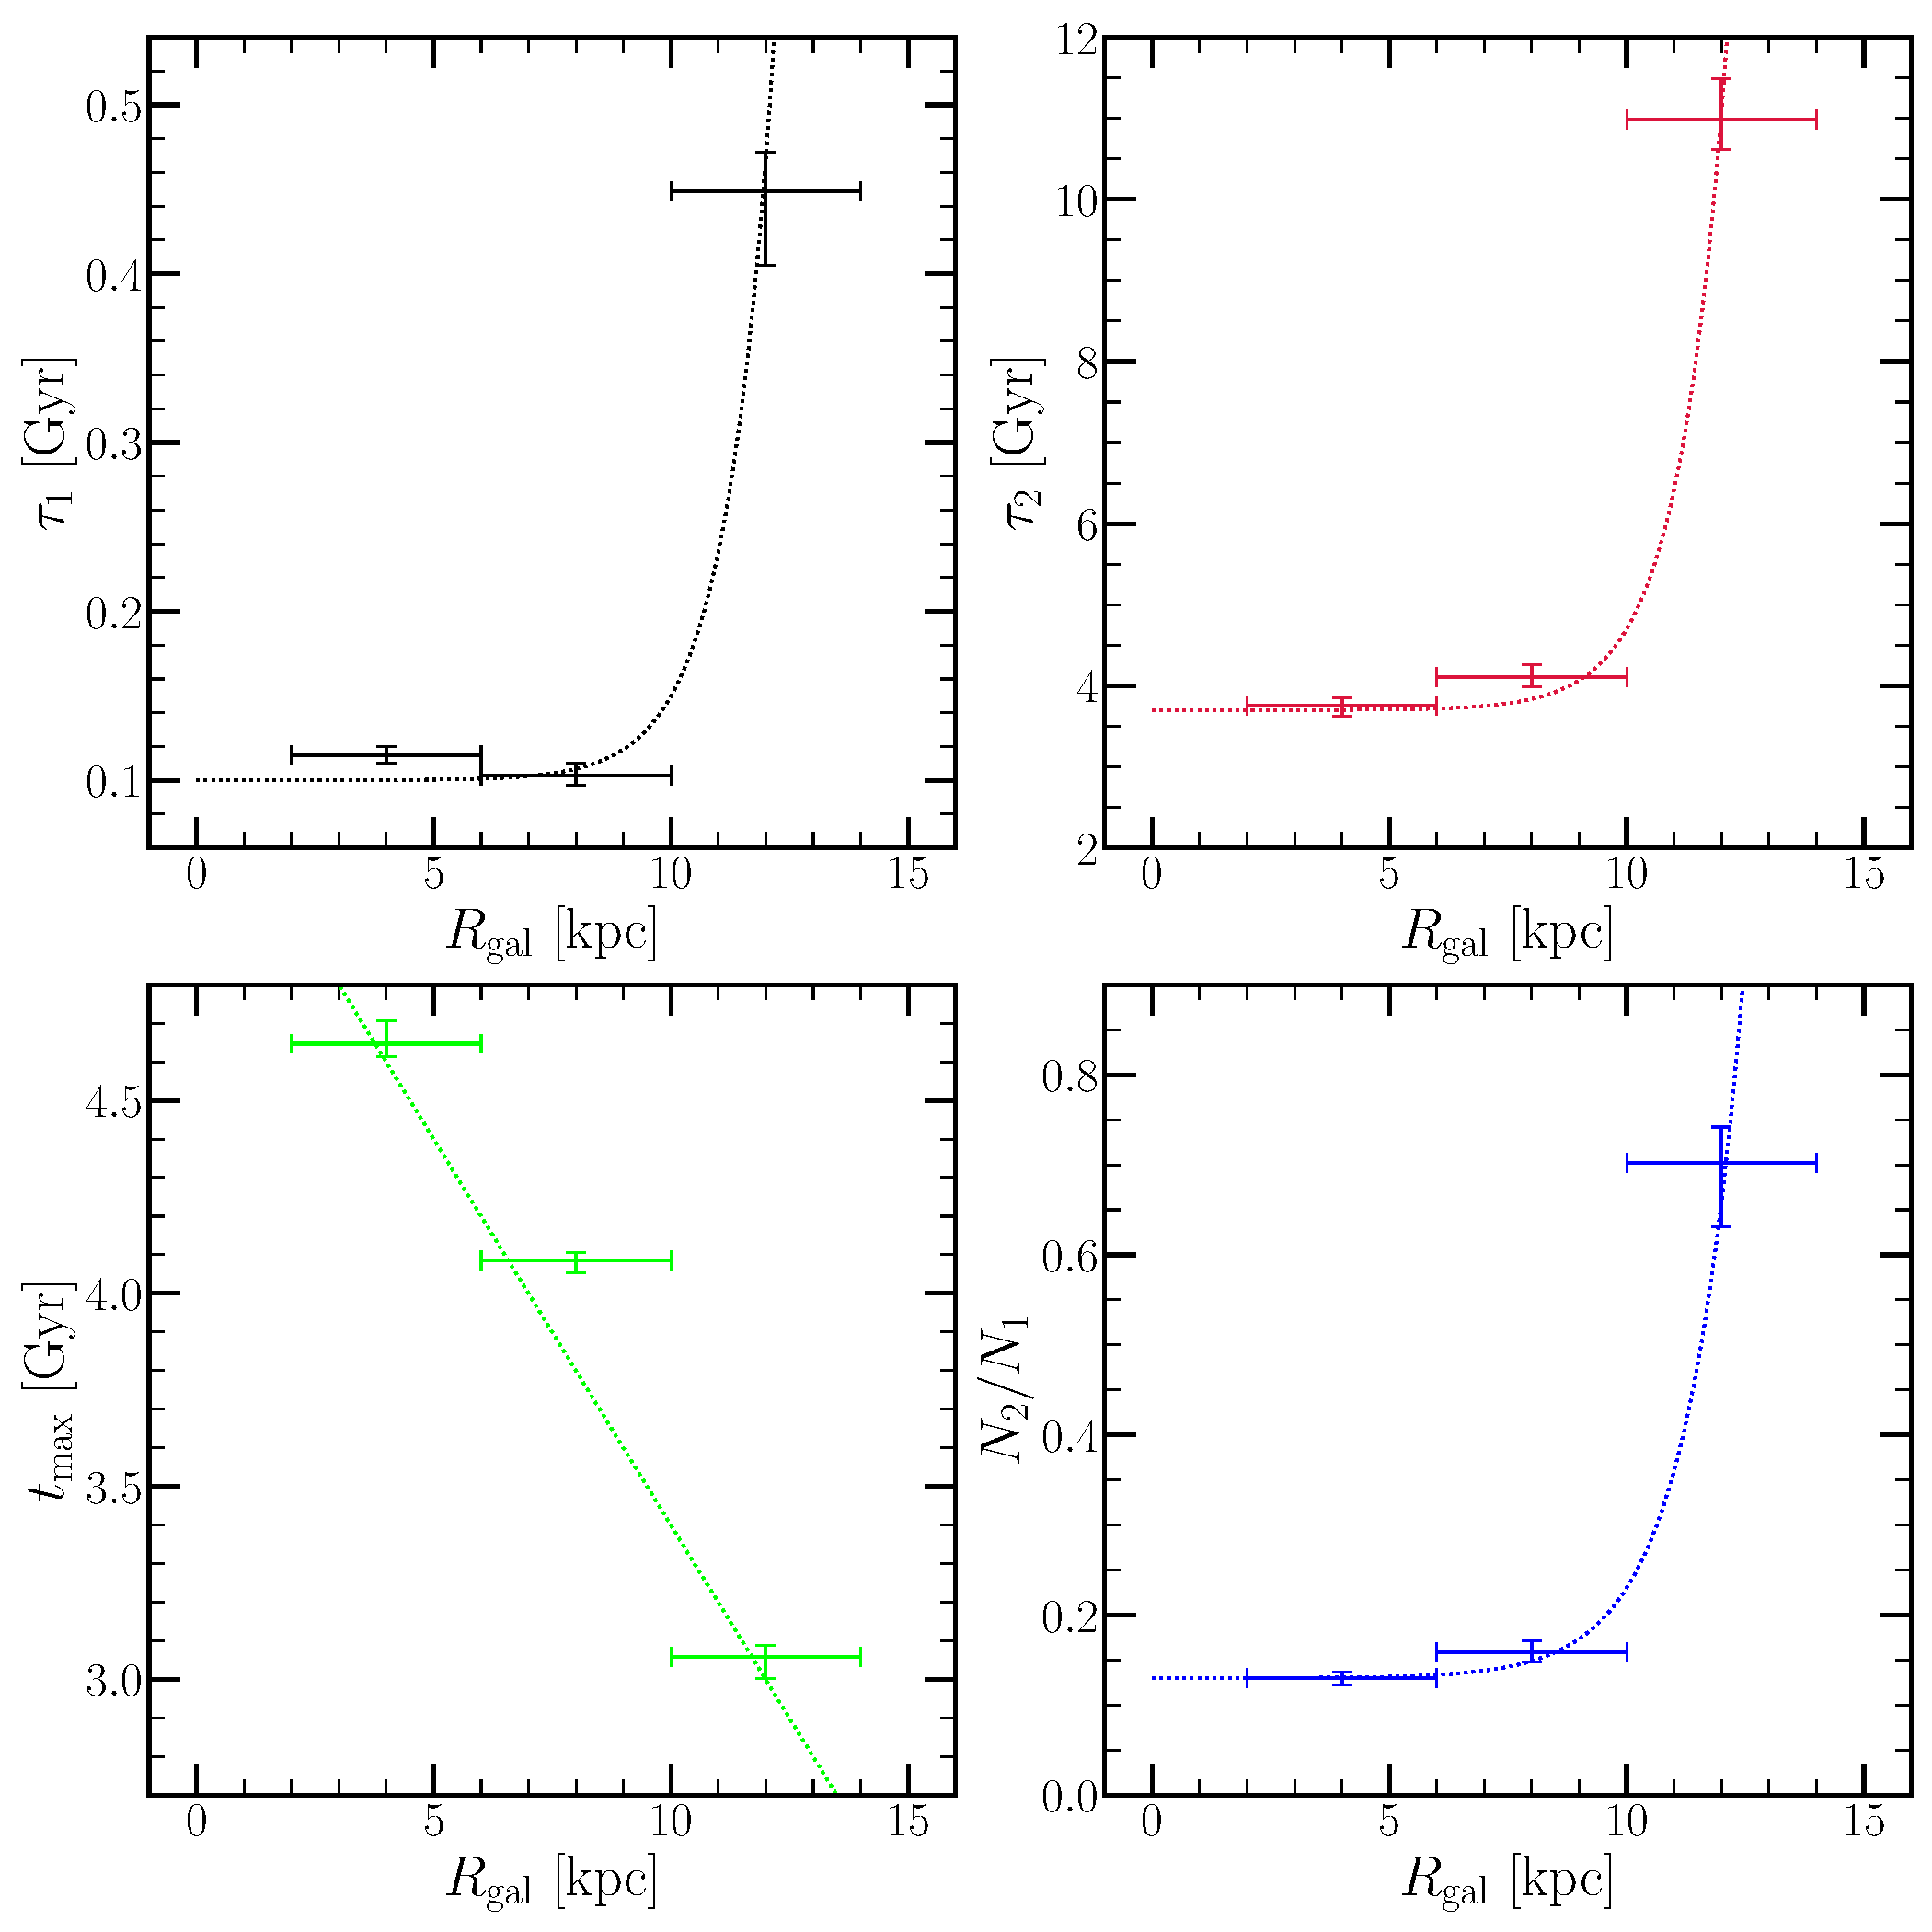
\includegraphics[scale = 0.35]{\main/parameters/spitoni2021_parameters.pdf} 
\caption{
Two-infall model fit parameters from~\citet{Spitoni2021}. 
Error bars denote the width of the annulus in their multi-zone model 
(x-direction) and the uncertainties on the parameter fit (y-direction). 
Dotted lines denote by-eye descriptions of the trends with~\rgal. 
The fit parameters are the e-folding timescale of the first infall episode 
(upper left), the e-folding timescale of the second infall episode (upper 
right), the time of onset of the second infall episode (lower right), and the 
ratio of amplitudes of the second to the first exponential describing the 
infall history (lower right). 
}
\label{fig:spitoni2021_parameters} 
\end{figure*} 

Fig.~\ref{fig:spitoni2021_parameters} plots the~\citet{Spitoni2021} fit 
parameters as a function of~\rgal, with a by-eye description of the trends 
shown in a dotted line. They are given by: 
\begin{subequations}\begin{align} 
\frac{\tau_1}{\text{Gyr}} &= 0.1 + e^{(\rgal - 13\text{ kpc}) / 1\text{ kpc}} 
\\ 
\frac{\tau_2}{\text{Gyr}} &= 3.7 + e^{(\rgal - 10\text{ kpc}) / 1\text{ kpc}} 
\\ 
\frac{\tmax}{\text{Gyr}} &= 5.4 - \frac{\rgal}{5\text{ kpc}} 
\\ 
\frac{N_2}{N_1} &= 0.13 + 0.1 e^{(\rgal - 10\text{ kpc}) / 1.2\text{ kpc}}  
\end{align}\end{subequations} 
In general, all parameters except~\tmax~are relatively constant within~$\sim$10 
kpc, beyond which they increase very quickly. 
The high values of~$\tau_1$ and~$\tau_2$ at large~\rgal~mean that at these 
radii, the SFH will resemble a step function more so than a double exponential. 
The high values of~$N_2/N_1$ indicate that the in-situ population there will 
overwhelmingly consist of young stars formed during the second infall episode. 
The negative slope of the~\tmax-\rgal~relation means that the second infall 
episode started earlier at large~\rgal~and propogated inward. 

\biblio 
\end{document} 

